\section{Integration}
To be able to simulate the particles with more precision, we have implemented multiple integration schemes. This has been done, since the euler method is very unstable and can explode very fast. Therefore we have implemented the following integration schemes:
\begin{itemize}
  \item[-] Euler, convert current force to acceleration and apply acceleration to current velocity weighted by the current time-step. Then update the position by the new velocity again weighted by the current time step.
  \item[-] Mid-Point, firstly backup the positions and velocities of the current particles. Then for each particle, calculate a intermediate velocity using the euler method and calculate the midpoint position with half the current time step. Then take another euler step from the midpoint. Finally restore the original position of all the particles and update the positions by the new midpoint velocity weighted by the the time step.
  \item[-] Runge-Kutta 4-order, similar to midpoint, but forces and constraints are evaluated four times. After each evaluation, the position of all the particles are reset and updated according to the new velocities calculated during the previous force/constraint evaluation, weighted by a fraction of the timestep. The final velocity is calculated by $v_f = v_{t0} + \frac{v_{k_1}}{6} + \frac{v_{k_2}}{3} + \frac{v_{k_3}}{3} + \frac{v_{k_4}}{6}$, where $v_{k_x}$, is the velocity of the particles after the $xth$ evaluation. In the end, the positions of each particles is again updated by the final velocity weighted by the time step.
\end{itemize}
The difference of the integration schemes can be notices easily. As displayed below, the Runga Kutta method is more stable than euler. Furthermore, we noticed that for our configuration, that the midpoint integration method was a little more stable than euler. Euler method easily explodes at around time-step 0.03 with interaction, but midpoint also exploded quite easily with interaction with time-step 0.039 by using interaction. Runga kutta start exploding with lots of interaction when using time-step 0.069s.

\begin{figure}[!htbp]
  \begin{subfigure}[h]{\textwidth}
  \centering
    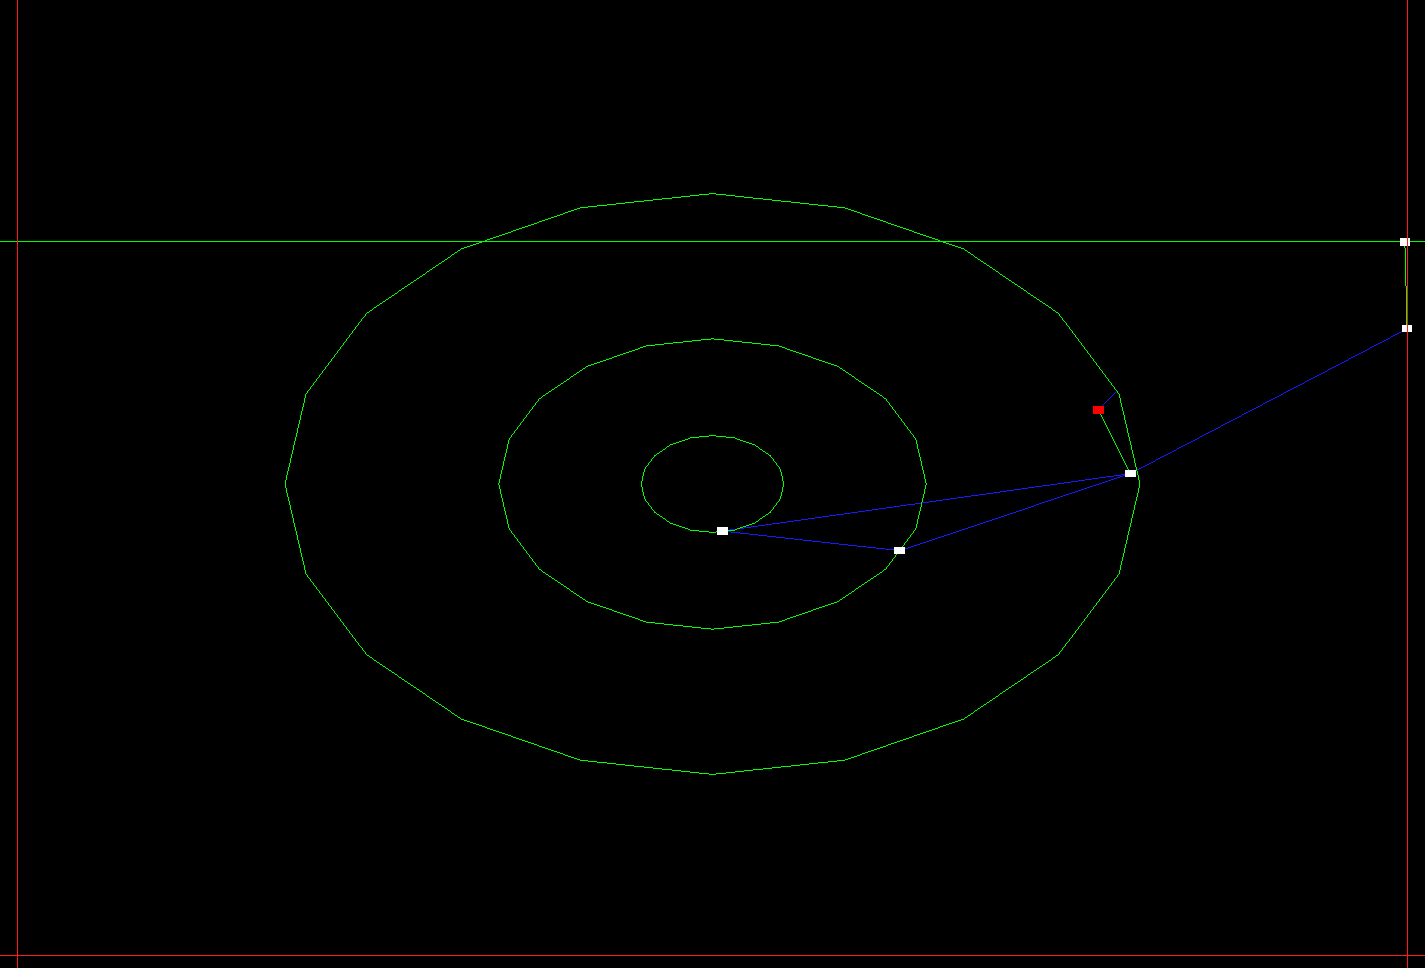
\includegraphics[width=0.4\textwidth]{euler1}
    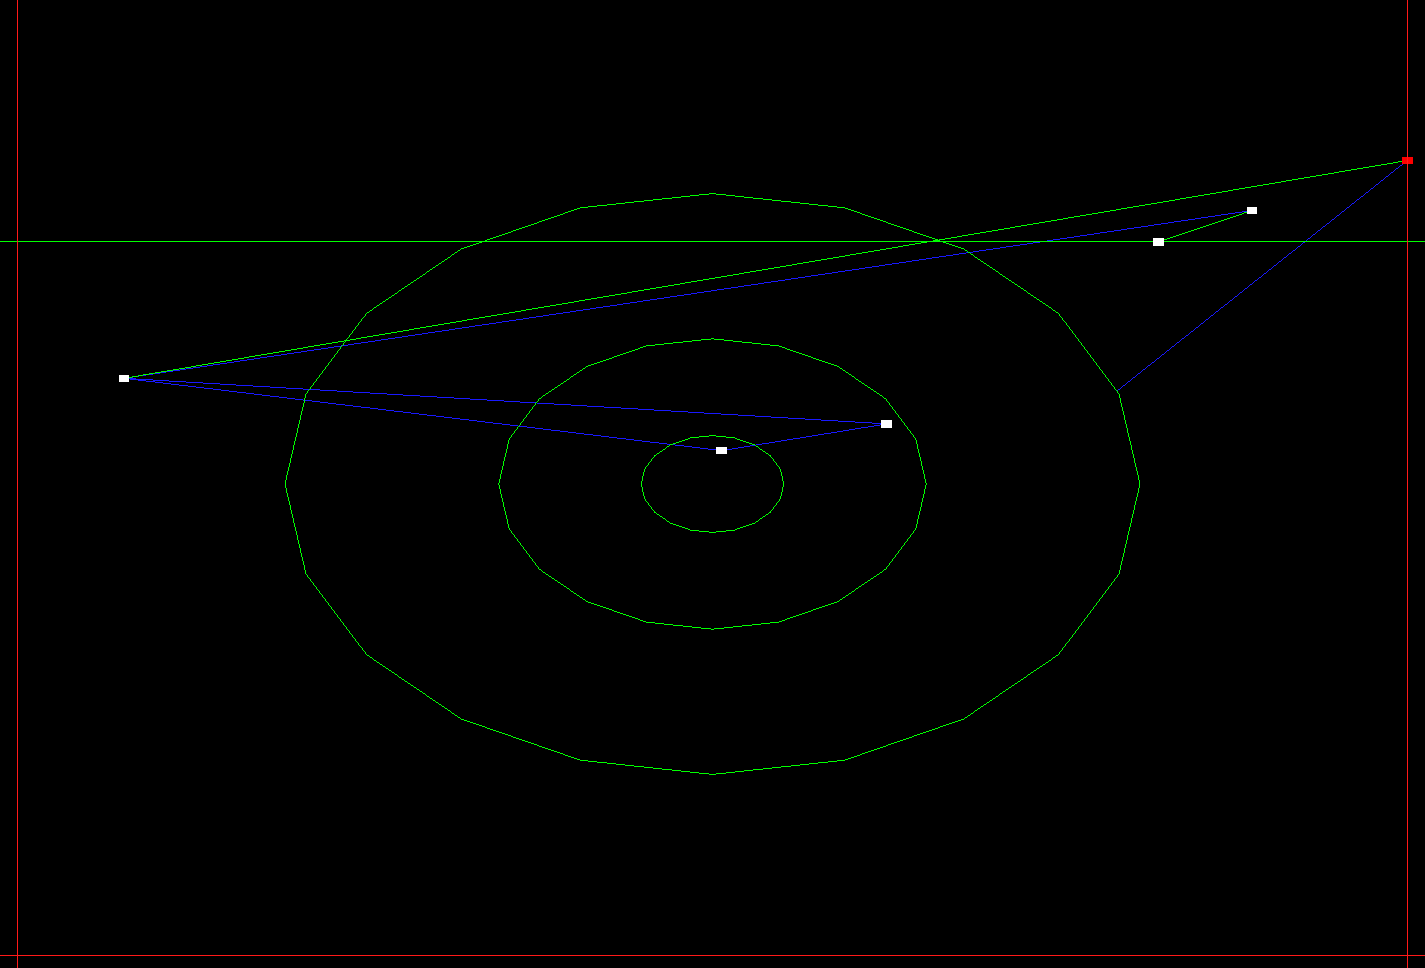
\includegraphics[width=0.4\textwidth]{euler2}
    \caption{Euler integration explodes after short time at time-step 0.04s}
    \label{fig:euler}
  \end{subfigure}
  \\
  \begin{subfigure}[h]{\textwidth}
  \centering
    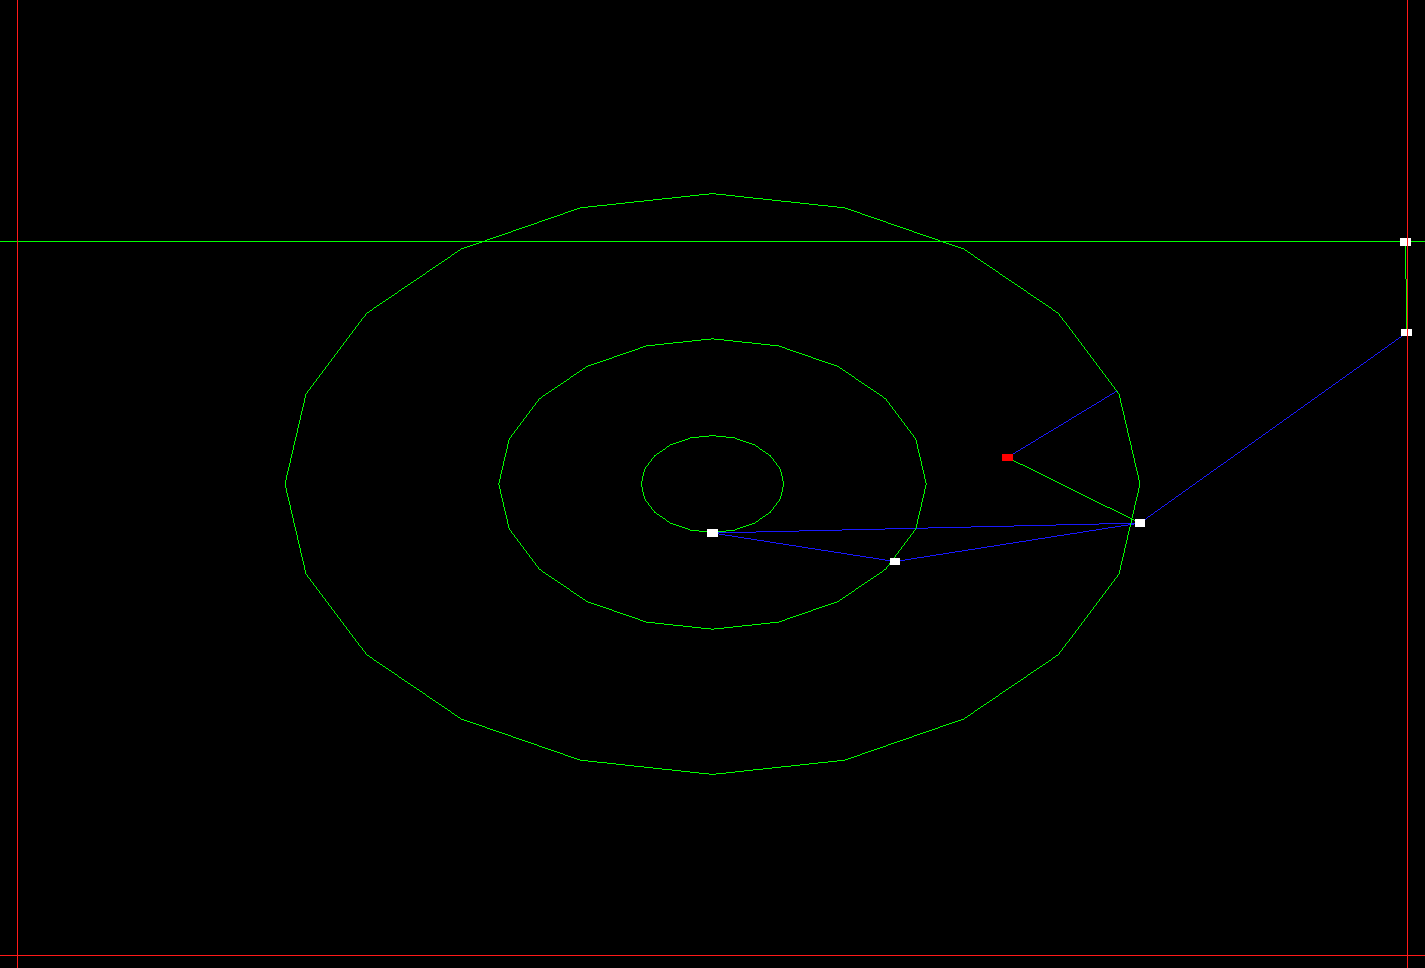
\includegraphics[width=0.4\textwidth]{runga1}
    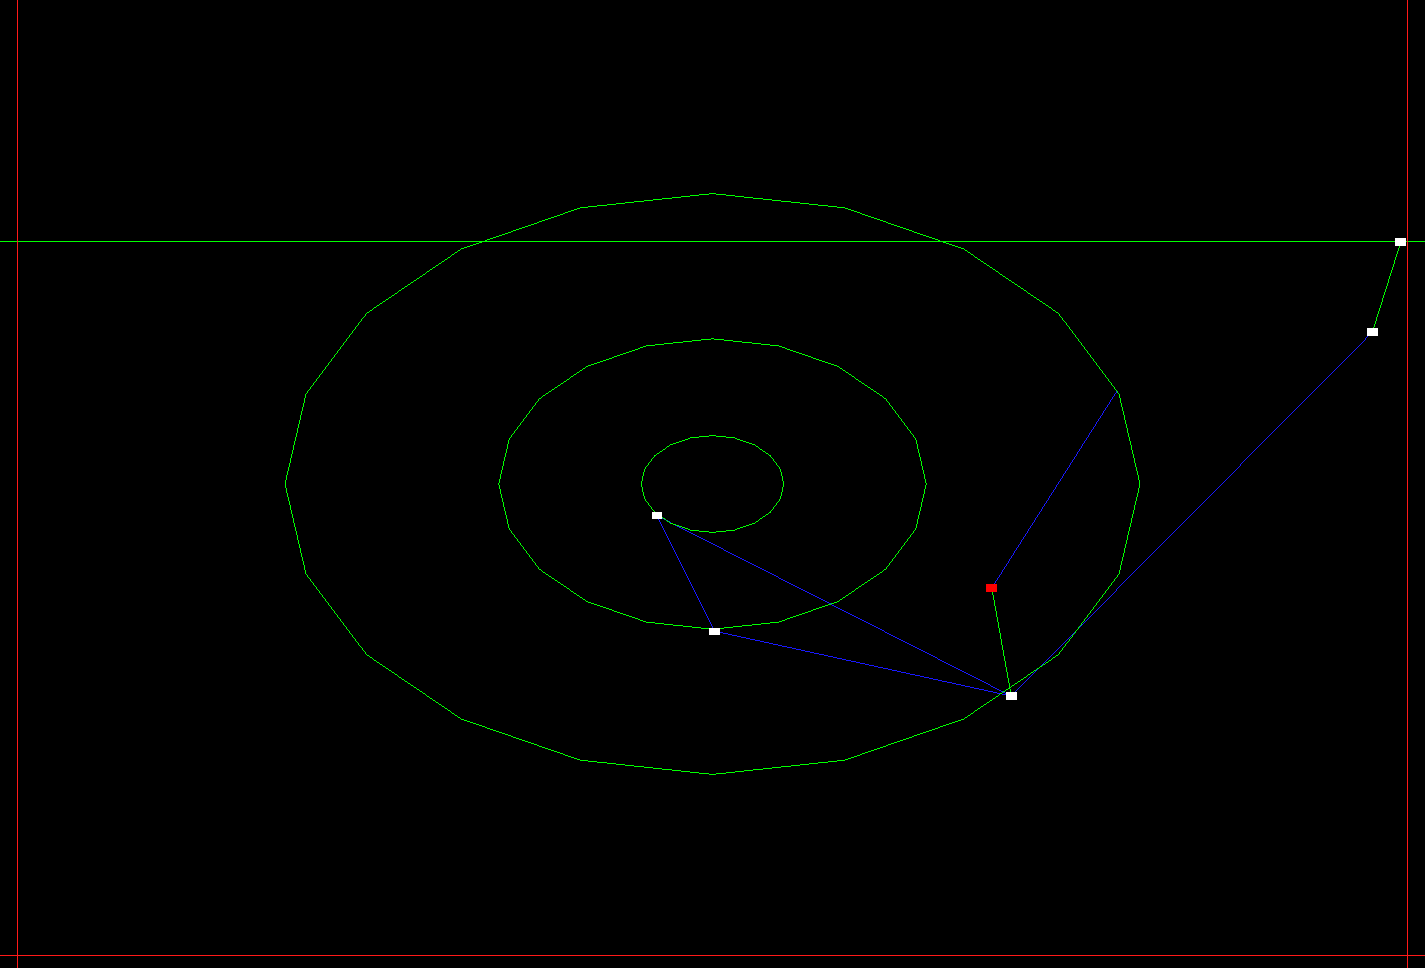
\includegraphics[width=0.4\textwidth]{runga2}
    \caption{Runga Kutta integration stays stable at time-step 0.04s}
    \label{fig:ruga}
  \end{subfigure}

  \caption{Comparison Euler and Runga Kutta integration scheme}
  \label{fig:integration}
\end{figure}
